%!TEX root = proj_report_outline.tex
\chapter{Evaluation}
Following the completed implementation and infrastructure setup an evaluation of the project was carried out on prototype. The evaluation was designed primarily to verify whether or not the prototype developed was successful in fulfilling the requirements identified as in scope in Section \ref{S:evaluationScope}.

\section{Test \rom{1} - Collaboration Functionality Fulfilment}

\subsection{Motivation}
PitchHub's primary goal is to facilitate collaboration within the innovation community. To do this PitchHub seeks to engage all roles in the innovation community by focusing de-constructing ideas to appeal their expertise - in terms of  value proposition, business opportunity, challenges, and solution. Test \rom{1} seeks to verify that the prototype supports the behaviour necessary to facilitate this collaboration. As discussed in Section \ref{C:requirements} this behaviour is distilled in the requirements D1, D2.1 and D2.2.

\subsection{Results}
The user stories which affirm the fulfilment of requirements D1, D2.1 and D2.2 in \textit{TB1} confirm support of the following behaviour:

\paragraph{Requirement D1's user stories specify the ability to:} post Pitch Cards, make suggestions on Pitch Points, accept/reject suggestions, comment on Pitch Points, comment on suggestions and mark Pitch Cards as completed/active.

\paragraph{Requirement D2.1's user stories specify the ability to:} scope entities such as Pitch Cards, suggestions, and one's identity such that unintended viewers are avoided. To ensure the completeness of these user stories, each scope/viewer level combination is tested. These combinations are displayed in Fig \ref{fig:architecturescope_matrix_evaluation}.

\begin{figure}[ht]
    \centering
    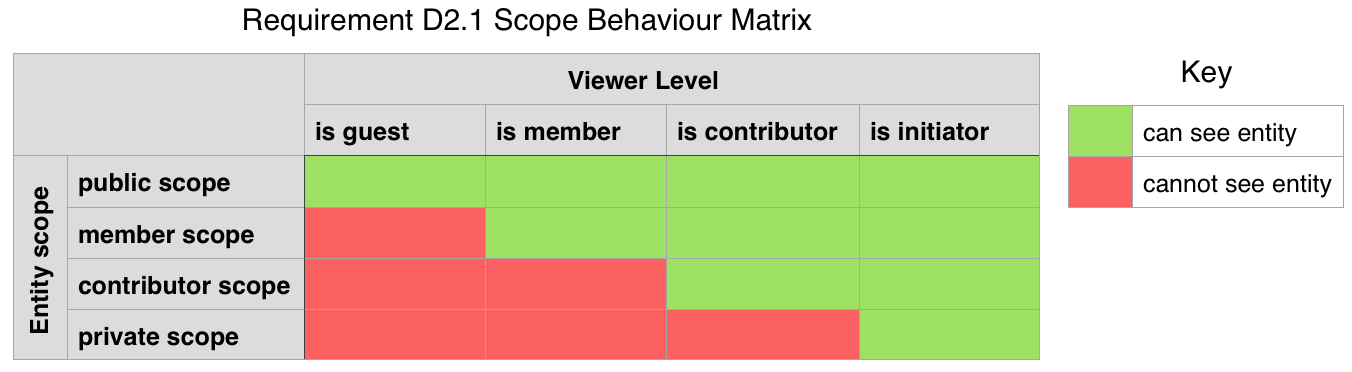
\includegraphics[width=1\textwidth]{scope_matrix}
    \caption{The scope matrix which illustrates the relationship between viewer level and entity scope in regards to viewing the entity.}
    \label{fig:architecturescope_matrix_evaluation}
\end{figure}

\paragraph{Requirement D1's user stories specify that:} users who have viewed a Pitch Card are able to be seen as a ``viewer'' by the PitchCard's initiator.

\subsection{Discussion}
The design of this experiment was guided by two main questions: first, ``what behaviours are needed to facilitate collaboration in the innovation community?'' And second, ``how can these behaviours be verified as functional from a user's point of view?''. In regards to the first question, determining what behaviours were required was to an extent already completed by Callaghan Innovation through their conceptualisation of PitchHub. To formalise these behaviours Callaghan Innovation and I collaborated on the specification of the user stories.
In regards to the second question, realistically simulating user interaction was identified as key. Manually testing the various behaviours and scope combinations would be time-consuming and tedious. \textit{TB1} automates this simulation with the added benefit of assertions, making it easy to verify that expected behaviour is indeed satisfied.
Concluding on the fulfilment of requirements D1, D2.1 and D2.2 largely relies on whether the behaviours specified in relation to the first question accurately reflects the behaviour required by the innovation community. Generalising what a large population needs is a difficult task but it is my belief that because the user stories tested were created in collaboration with Callaghan Innovation, who is a large participant in the innovation community, they are therefore meet the level of credibility required for the purposes of this test. As such, it is concluded that requirements D1, D2.1 and D2.2 have been fulfilled.

\section{Test \rom{2} - Deployed Prototype Analysis}
At the time of writing, the prototype, \textit{TB3}, has been successfully been released to Callaghan Innovation and is ready for use. Unfortunately use of the prototype by Callaghan Innovation has not yet fully commenced. Without substantial activity to analyse this test was unable to be completed. It is expected that the access code will be distributed by the Callaghan Innovation stakeholders to the wider organisation in the coming weeks.

\section{Test \rom{3} - Community Size Support}

\subsection{Motivation}
Supporting collaboration within the innovation community firstly requires that sheer size of the community is able to be supported. Test \rom{3} seeks to test whether the PitchHub prototype could support the entire NZ innovation community. The sizes tested against are derived from the Statistics NZ data, where the expected size is estimated to be a population of 437,403 and the worst case size is estimated to be a population of 589,340.

Test \rom{3} uses the prototype in a diverse ``3, 4'' secret sharing scheme configuration (2x MongoDB replica sets and 2x Postgres instances).

\subsection{Results}

\subsection{Discussion}

\section{Test \rom{4} - Overhead of Threshold Scheme Security}

\subsection{Motivation}
The secret sharing service is an important part of keeping sensitive user data secure. A consequence of this service is a loss of performance - through the latency introduced by the queries to the secret keepers and added processing to reconstruct secrets. Test \rom{4} seeks to measure the overhead of this service and discuss whether the security afforded is worth the performance loss.

Test \rom{4} uses the prototype in both a non-secret sharing configuration (1x MongoDB replica set) and a diverse ``3, 4'' secret sharing scheme configuration (2x MongoDB replica sets and 2x Postgres instances).

\subsection{Results}

\subsection{Discussion}

\section{Test \rom{5} - Overhead of Secret Keeper Diversity}

\subsection{Motivation}
To strengthen the security afforded by the secret sharing service diversity was added to the secret keepers. A consequence of this is that the service is now only as fast as it's slowest secret keeper. Test \rom{5} seeks to measure the overhead of this added diversity and discuss whether the extra security afforded is worth the performance loss.

Test \rom{5} uses the prototype in a both a diverse ``3, 4'' secret sharing scheme configuration (2x MongoDB replica sets and 2x Postgres instances) and a homogeneous ``3, 4'' secret sharing scheme configuration (4x MongoDB replica sets).

\subsection{Results}

\subsection{Discussion}


\section{General Discussion}
@KB, not sure if this section will be necessary

The disadvantage of unconditionally secure secret sharing schemes is that the storage and transmission of the shares requires an amount of storage and bandwidth resources equivalent to the size of the secret times the number of shares. If the size of the secret were significant, say 1 GB, and the number of shares were 10, then 10 GB of data must be stored by the shareholders
